% !TEX TS-program = pdfLaTeX
% !TEX encoding = UTF-8

\documentclass[12pt]{article}  % tipo de documento

\usepackage[utf8]{inputenc}  % levar em consideração que é um arquivo em utf8
\usepackage{times}                 % um fonte que tenha acentos
\usepackage[T1]{fontenc}      % levando em consideração utf8 na hora de escolher as letras da fonte
\usepackage{hyperref}
\usepackage{fancyhdr}           % manipular o cabeçalho
\usepackage[normalem]{ulem} % sublinhado que não sobreescreve \emph
\usepackage{tikz}

% http://sourceforge.net/projects/pgfplots/
\usepackage{pgfplots}

%\usepackage{pstricks}
%\usepackage{pst-plot}

\pagestyle{fancy}
\setcounter{tocdepth}{5}

\rhead{Desenhando no \LaTeX}

\begin{document} 

% Introduce a new counter for counting the nodes needed for circling
\newcounter{nodecount}
% Command for making a new node and naming it according to the nodecount counter
\newcommand\tabnode[1]{\addtocounter{nodecount}{1} \tikz \node (\arabic{nodecount}) {#1};}

% Some options common to all the nodes and paths
\tikzstyle{every picture}+=[remember picture,baseline]
\tikzstyle{every node}+=[inner sep=0pt,anchor=base,
minimum width=1.8cm,align=center,text depth=.25ex,outer sep=1.5pt]
\tikzstyle{every path}+=[thick, rounded corners]

\title{\LARGE 
	Desenhando no \LaTeX 	
}
\maketitle

%\tableofcontents

\section{} 
\begin{tabular}{|  l  | c | r | }
  \hline                       
  1 & \tabnode{2} & 3 \\ \hline
  4 &  5 & 6   \\ \hline
  7 & \tabnode{8} & 9 \\
  \hline  
\end{tabular}

\begin{tikzpicture}[overlay]
\draw [orange] (1.north west) -- (1.north east) -- (1.south east) -- (1.south west) -- cycle;

\node [right=2cm,above=2cm,minimum width=0pt] at (1) (A) {A};
\draw [<-,out=5,in=180] (1) to (A);
\end{tikzpicture}



% pfgplot package
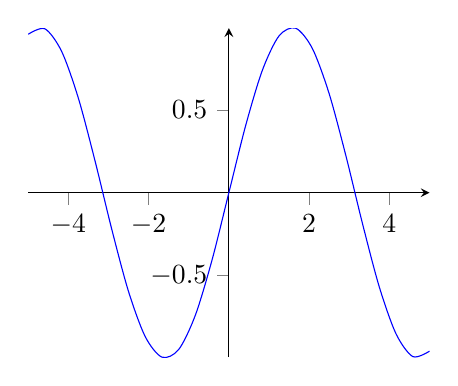
\begin{tikzpicture}
	\begin{axis}[width=190pt,axis x line=middle, axis y line=center, tick align=outside]
		\addplot+[mark=none,smooth] (\x,{sin(\x r)});
	\end{axis}
\end{tikzpicture}

%pst-plot
%\begin{pspicture}(-8,-2)(8,2)
%  \psgrid[griddots=10,gridlabels=0pt, subgriddiv=0, gridcolor=black!20]
% \psaxes(0,0)(-8,-2)(8,2)
% \psplot[linecolor=red, linewidth=2pt]%
%     {-8}{8}{x neg -1 atan 180 sub 180 div 3.1416 mul}
%\end{pspicture}


\subsection{}

\subsubsection{}

\subsubsection{Enumerados}


\end{document}











